\chapter{Canlyniadau}
Mae'r bennod hon yn cyflwyno disgrifiad o'r sesiynau prawf a gymerwyd gan brawfwyr dienw ar y llwyfan gwe. Gellir dod o hyd i'r holl god ar gyfer y canlyniadau a gyflwynir yma ar GitHub\footnote{Gweler y nodyn yn y cronfa ddata yn y cwmwl \url{https://github.com/Oktogazh/analeksis}}.

\section{Descriptive Statistics}
Ar adeg ysgrifenu, casglwyd cyfanswm o 171 sesiwn prawf. Yr oedd nifer cyfartalog yr allweddi (geiriau go iawn) ym mhob sesiwn yn 47.743. Gan fod llithiau yn disgwyl i nifer cyfateb i'r allweddiau, yr oedd nifer gyfartalog yr eitemau ym mhob sesiwn felly ychydig yn llai na chan. Fel atgoffa, mae hyd y sesiynau yn dibynnu ar sgôr y rhai sy'n cymryd y prawf. Po uchaf yw sgôr y prawf y gellir ei chyrraedd, mwyaf yw'r nifer o eiriau go iawn y ceir eu gweld. Mae'r cymhareb cyfartalog o lithiau a adnabuwyd (larymau ffug) yn 21.5\%, gyda chyfartaledd o 9 gair ffug a adnabuwyd mewn termau absoliwt. Mae'r gwerth olaf hwn yn ymddangos yn annisgwyl o'r diwedd a sbardunodd ymchwiliad pellach. Mae'r ffigur \ref{fig:score-fa} yn dangos dosbarthiad o sgôrion terfynol y sesiynau ynghyd â chymhareb y geiriau ffug a adnabuwyd.

Fel gellir gweld, hyd yn oed y sgôrion uchaf oedd â rhai achosion o larymau ffug, a dim ond ychydig o sgôrion isel sydd â chyfran sero. Mae hyn yn golygu bod y sgôrion terfynol uchaf hefyd yn rhai sesiynau gyda'r mwyaf o achosion o larwm ffug mewn termau absoliwt. Er gwaethaf bod hyn yn eithaf annisgwyl, mae'r ffaith bod larymau ffug yn cael eu hadnabod o bryd i'w gilydd gan yr holl ystod o sgorwyr yn annog. Yn gyntaf, mae hyn yn golygu bod y geiriau ffug wedi'u cynllunio'n dda, gan ddilysu'r cysyniad o ddefnyddio RNN i'w cynhyrchu. Hefyd, gellid sefydlogi taflwybr hir-dymor y larymau ffug trwy addasu'r disgwyliadau cyn ddiweddaru eu graddio yn y back-end. Drwy droi'r siawns i eitem gael ei hadnabod i fod bob amser yn gyfradd ffug bositif y sesiynau (yn hytrach na'r raddio terfynol fel ar gyfer yr allweddi), byddai graddio'r rhan fwyaf o eiriau ffug yn aros mewn ystod agos at rai geiriau ffug. Byddai'r larymau ffug gwael eu ffurfio'n disgyn i lawr mewn graddio a byddai'r rhai nad ydynt yn nonsensical yn codi mewn ffordd lle byddai'r ddau yn gorffen allan o'r amrediad. Nodwch nad yw'r nodwedd hon wedi'i gweithredu eto, er y byddai'n hawdd ei wneud yn dechnegol. Yr ystod gyfartalog o larwm ffug yw 207, hynny yw, gwahaniaeth gradd y llithiau uchaf ac isaf a adnabuwyd mewn sesiwn. Mae hyn i'w roi mewn persbectif gyda sgôr gyfartalog o 566. Mae hyn yn golygu bod larymau ffug wedi dechrau ar gyfartaledd pan fo siawns adnabod gair go iawn rhwng 75\% a 50\%. Felly mae siawns larymau ffug yn y cyfnod penodol hwn pan mae'r cynnydd yn dechrau arafu yn fwy na'r cyfartaledd o 21.5\% ar draws y sesiynau cyfan. Mae'r pwynt hwn yn amlygu anhawster modelu goddefgarwch i risg neu strategaethau twyllo posibl. Gallai hyn wneud y canlyniadau'n anghymharadwy rhwng proffiliau gwahanol, mwy ar hynny yn y bennod nesaf.

Sylw ôlaf, a llai o syndod, yw bod y rhan fwyaf o'r sesiynau, 142, yn dod o'r prawf llydaweg. Mae hyn oherwydd i'r profion eraill gael eu hychwanegu i'r llwyfan yn ddiweddarach. Yn amlwg, nid oes gan y profion Cymraeg, Wcreineg a Ffrangeg ddigon o ganlyniadau ar gyfer unrhyw ddadansoddiad difrifol. Dyma'r rheswm pam ein bod yn canolbwyntio ar sesiynau'r prawf Llydaweg yn yr adran ganlynol.

\begin{figure}
    \centering
    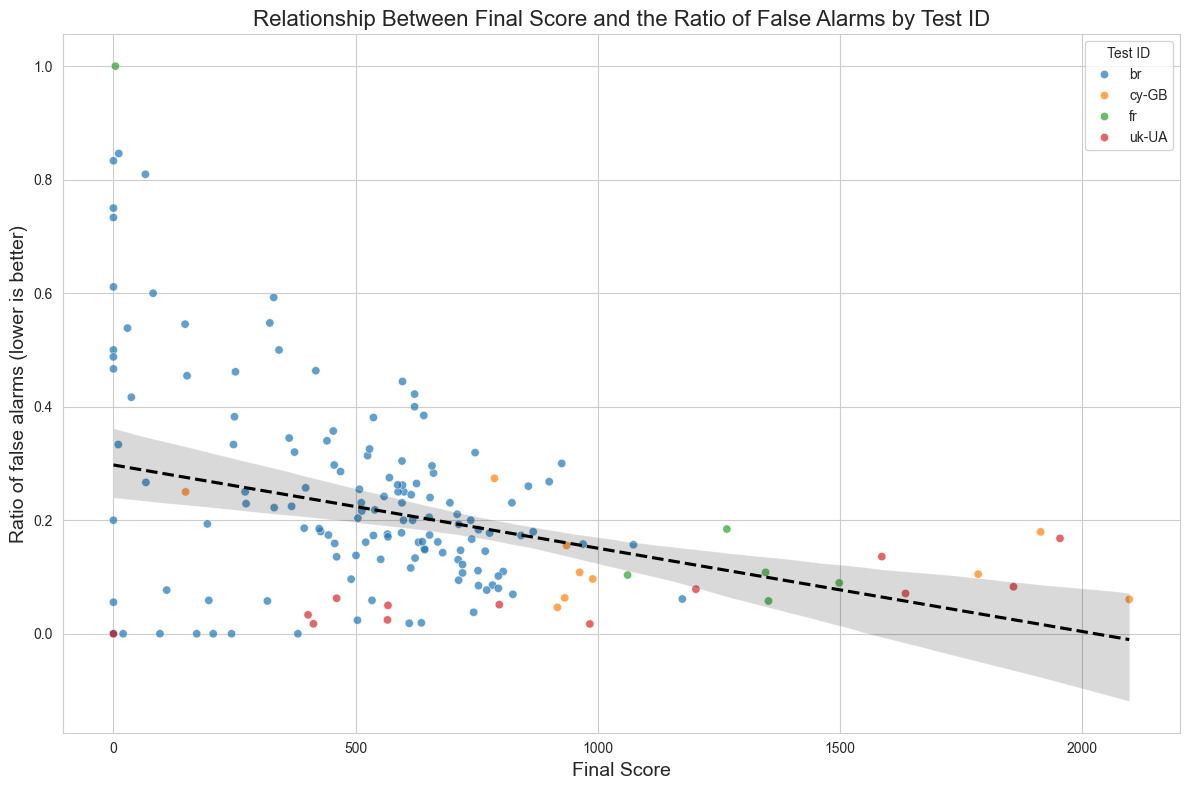
\includegraphics[width=0.8\linewidth]{figures/scores-fa.png}
    \caption{Dosbarthiad sgôrion ar draws sawl prawf a'u cyfraddau ffug positif cysylltiedig}
    \medskip
    \small
\end{figure}\label{fig:score-fa}

\section{Mesur Addasu}
Fel y soniwyd yn flaenorol, gallwn ddefnyddio'r gair go iawn olaf a adnabuwyd mewn sesiynau i brofi addasu. Y nifer o eiriau go iawn olaf a adnabuwyd yn rownd olaf prawf Llydaweg yw 73 o 142, sef 51.4\%. Os byddem yn ceisio profi'r rhagdybiaeth o gamgywiro system, byddai angen gwerth-p o dan 0.05. Fodd bynnag, mae rhedeg prawf binomial gyda'r canlyniadau hyn yn cynhyrchu gwerth-p o 0.801. Mae hyn yn uchel iawn, ac nid yw'n difwyno'r rhagdybiaeth anolo gysylltiedig bod siawns adnabod y gair go iawn olaf yn llawn ansicr. Mewn geiriau eraill, ni welwn unrhyw reswm i amau cywirdeb a dibynadwyedd y prawf.

Mae'r canlyniad hwn yn annog yn fawr mewn sawl ffordd. Yn gyntaf, dim ond tri chategori amlrwydd a ddefnyddiwyd i ymgychwyn gradd y geiriau go iawn yn y prawf. Mae hyn yn golygu bod y rhestrau amlrwydd hir ac adnodd-dwys yn bron yn angenrheidiol, sy'n werthfawr mewn cyd-destun IAC. Mae'r buddion o ddefnyddio'r dechneg clystyrau modulo i greu system hybrid rhwng cyfran yr atebion cywir a graddfa logistaidd glasurol yn cael eu cysuro. Yn ail, mae lefel y cywirdeb a honnir yn uchel iawn. Mae'r cywirdeb yn cael ei ddiffinio gan y ffwythiant ansicrwydd \ref{eq:uncertainty-function}. Mae'n amrywiol, oherwydd ei bod yn dibynnu ar nifer yr eiriau go iawn a welwyd yn y sesiwn, nifer sy'n dibynnu ar hyd y sesiwn, sy'n dibynnu ar y cynnydd graddio. Ysywaeth, ni chaeth eu storio gwerthau olaf yr ansicrwydd ar gyfer y sesiynau, ond gwys nid yw i fod yn uwch na ±52, ac bydd yn fwy yn y sesiynau hiraf.

Gan oedd y canlyniadau cynnar ar brofi addasu'r prawf yn annog, rydym yn cynnig ehangu'r dadansoddiad i ystodau penodol. Rhoddir y canlyniadau yn y tabl~\ref{tab:recognition_stats}.

\begin{table}[h]
\centering
\begin{tabular}{|c|c|c|c|c|}
\hline
\textbf{Ystod} & \textbf{Sesiwnau} & \textbf{Geiriau Adnabuwyd} & \textbf{Cyfartaledd} & \textbf{Gwerth-p} \\
\hline
(0, 100] & 10 & 6 & 0.600000 & 0.753906 \\
(100, 200] & 7 & 1 & 0.142857 & 0.125000 \\
(200, 300] & 7 & 2 & 0.285714 & 0.453125 \\
(300, 400] & 12 & 6 & 0.500000 & 1.000000 \\
(400, 500] & 14 & 6 & 0.428571 & 0.790527 \\
(500, 600] & 29 & 16 & 0.551724 & 0.711071 \\
(600, 700] & 22 & 12 & 0.545455 & 0.831812 \\
(700, 800] & 22 & 13 & 0.590909 & 0.523467 \\
(800, 900] & 7 & 6 & 0.857143 & 0.125000 \\
(900, 1000] & 8 & 3 & 0.375000 & 0.726562 \\
(1000, 1100] & 2 & 1 & 0.500000 & 1.000000 \\
(1100, 1200] & 1 & 1 & 1.000000 & 1.000000 \\
(1200, 1300] & 2 & 0 & 0.000000 & 0.500000 \\
(1300, 1400] & 2 & 2 & 1.000000 & 0.500000 \\
(1400, 1500] & 1 & 0 & 0.000000 & 1.000000 \\
(1500, 1600] & 1 & 0 & 0.000000 & 1.000000 \\
(1600, 1700] & 1 & 0 & 0.000000 & 1.000000 \\
(1700, 1800] & 1 & 1 & 1.000000 & 1.000000 \\
(1800, 1900] & 1 & 0 & 0.000000 & 1.000000 \\
\hline
\end{tabular}
\caption{Cyfartaledd y gair go iawn olaf a adnabuwyd mewn ystodau penodol o sgôrion terfynol y prawf Llydaweg, gyda gwerthoedd-p o dest binomial}
\label{tab:recognition_stats}
\end{table}

Gellir gweld bod y canlyniadau yn bennaf yn gyson â 50\% siawns o gael adnabod y geiriau go iawn olaf. Nodwch fod y dull hwn yn ymddangos yn gallu dangos arwyddion cynnar o effeithiau silff posibl. Mae'r trawsnewidiad o dan i uwch na 900 yn ymddangos yn dangos effeithiau nenfwd posibl. Mae'r ystod 800–900 yn cael cyfartaledd uwch na 85\%, tra bod yr ystod 900–1000 yn gostwng i 37\%. Unwaith eto, mae maint y sampl yn rhy fach i gadarnhau presenoldeb effeithiau nenfwd sylweddol. Ond gallai'r dull dadansoddi hwn ddangos problemau o'r fath pe defnyddid prawf ar raddfa fwy. Ar y llaw arall, byddai mabwysiadu ehangach o'r prawf yn gwella'r calibriad, a thrwy hynny'n gwella'r canlyniadau.